\documentclass[a4paper,twoside]{report}

\usepackage{geometry}
\usepackage{multicol}
\usepackage{caption}
\usepackage{graphicx}
\usepackage{pgf}
\usepackage{multirow}
\usepackage{wrapfig}
\usepackage{indentfirst}
\usepackage{setspace}
\usepackage{amsmath}
\usepackage{mathtools}

\geometry{
	top=2cm,
	bottom=2cm,
	left=2cm,
	right=2cm,
}
\graphicspath{{./img/}}
\setlength{\columnseprule}{1pt}

\newenvironment{Figure}
  {\par\medskip\minipage{\linewidth}}
  {\endminipage\par\medskip}

\begin{document}
    {\large Lab 5: Operational Amplifiers }
    \hfill
    {\large \textbf{Pre-Lab 03-C-05} \par}
	\vspace{0.1in}
    {\large AmirHossein Habibvand - 810196447}
    \hfill
    \today \par
    {\large Nima Modares Gorji - 810196558 \par}
	\vspace{0.5in}

    \section*{Part 1}
    {
        \setstretch{1.5}
        \begin{figure}[!h]
            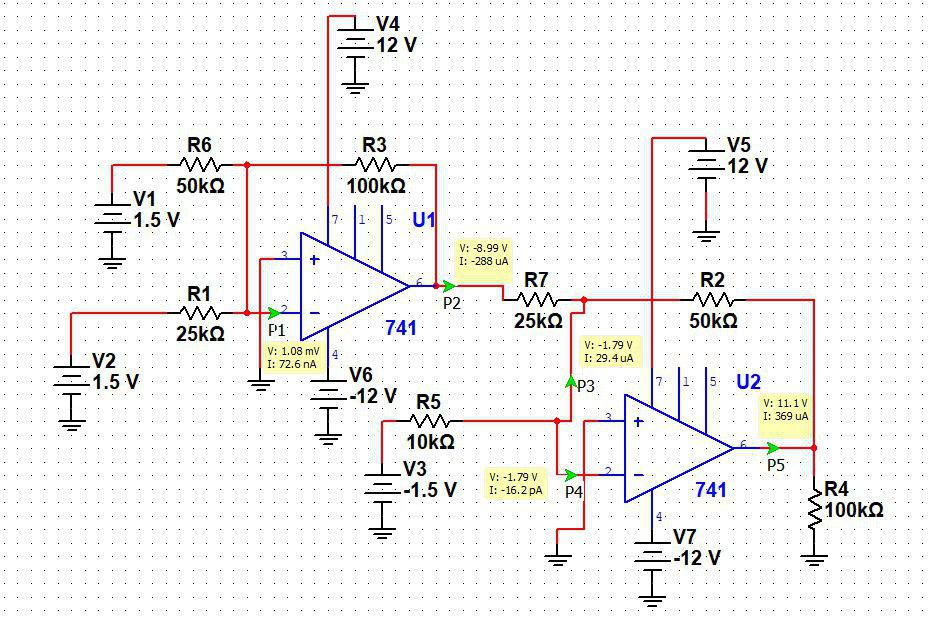
\includegraphics[width=\linewidth]{part1.jpg}
            \caption{Circuit 1 Schema}
            \label{fig:part1}
        \end{figure}

        As shown in Figure \ref{fig:part1}, in op-amp $U_1$, $V_{in_+}$ and $V_{in_-}$ are equal and $V_{S_-} < V_{out} < V_{S_+}$.

        But in op-amp $U_2$, $V_{in_+} \neq V_{in_-}$ so op-amp $U_2$ is in its nonlinear region and is saturated and $V_{out}$ is almost equal to $V_{S_+}$.

        op-amp in linear region: $V_{out} = A * (V_{in_+} - V_{in_-})$ where A is op-amp gain.

        op-amp in nonlinear region: $V_{out} \simeq V_{S_+}$
    }

    \newpage

    \section*{Part 2}
    {
        \setstretch{1.5}
        \begin{figure}[!h]
            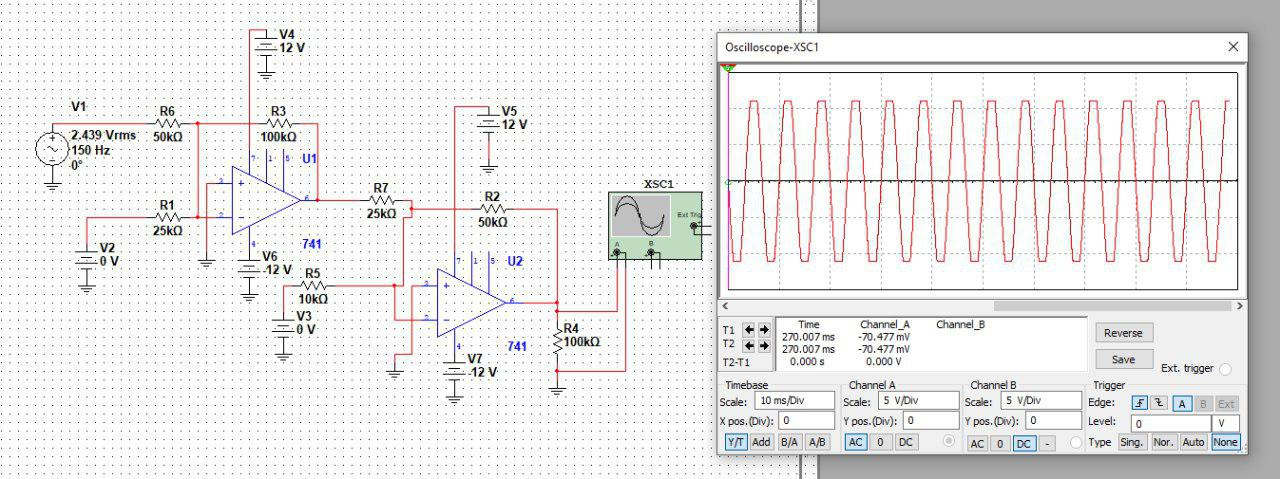
\includegraphics[width=\linewidth]{part2.jpg}
            \caption{Circuit 2 Schema with oscilloscope}
            \label{fig:part2}
        \end{figure}

        As shown in Figure \ref{fig:part2}, $V_2 = V_3 = 0$ and $V_{rms}$ of $V_1$ is equal to $2.439 V$.

        The oscilloscope shows the voltage waveform.

        Current waveform can be obtained from this equation: $V_{R_4} = i_0 * R_4, R_4 = 100k\Omega$.

        As the resistor $R_4$ is constant, so overall waveforms of current and voltage of the resistor are the same.
  }

\end{document}
